%%%%%%%%%%%%%%%%%%%%%%%%%%%%%%%%%%%%%%%%%%%%%%%%%%%%%%%%%%%%%%%%%%%%%%%%
\section{Contributions}
\label{sec:1_3_1_goal}

The research carried out during this thesis aims to contribute to the scientific community by designing heuristic and optimization-based ensembles. Consequently, small-size and effective ensembles could be designed. Below, the main contributions of this thesis are briefly discussed:

\begin{itemize}

    \item \textbf{Training set selection and swarm intelligence:} To alleviate the computation complexity associated with training large-size ensembles. In this proposal, we prove the possibility of building MCS from a reduced portion of training data. While to reduce the randomness of data sampling, intelligent data sampling in the form of instance selection is used. Regarding that, the ensemble members could focus deeply on the most informative data samples during the train. Furthermore, the combination function could be optimized via the search capabilities of SI algorithms. In this case, a class-specific weight is assigned to each classifier based on its accuracy to predict different samples from each class.
    
    \item \textbf{A guided search for ensemble pruning:} The small-size ensembles have benefits; save the testing time, reduce memory burden, reduce the communication costs of distributed models, and improve the prediction accuracy. While it is not easy to prune from overproduced ensembles. In this proposal, we discuss efficient and critical heuristic metrics for ensemble pruning. In addition, a guided search is presented for handling the conflicting of those metrics to enhance the general accuracy of subset integration. The pruning process starts after the individual's accuracy and the ensemble diversity are captured in a preliminary search set. In connection with our first contribution, the efficiency of ensemble systems can be further improved during the learning phase, by fast learning from reduced samples, and during the testing phase, by reducing the ensemble size via guided search. For that, our contribution is to downsize the training data and to downsize the classifiers simultaneously without affecting the performance of MCS.
     \item \textbf{An analysis of heuristic metrics for classifier ensemble pruning:} MCSs are superior to any random single classifier. However, three main defects are reported for those systems; (1) A large pool of classifiers should be built, (2) A sufficient memory space should be available to store those models, and (3) A large classification time will be consumed for combining multi-decisions. To alleviate these drawbacks, we discuss the concept and the benefits of thinning/pruning ensemble of classifiers. An effective, fast, and implementable heuristic metrics are analyzed to reorder the classifier's position in the generated random bagging. The investigated metrics are based on modifying the order of the classifiers in the bagging algorithm with the selection of the first set in the queue. Some of these criteria include general accuracy, complementary decisions, ensemble diversity, the margin of samples, minimum redundancy, discriminant classifiers, and margin hybrid diversity. The efficacy of those metrics is affected by the original ensemble size, the required subensemble size, the kind of individual classifiers, and the number of classes. While the efficiency is measured in terms of the computational cost and the memory space requirements. The separate performance of those metrics is assessed over binary and multiclass benchmark classification tasks, respectively.  In addition, the behavior of those metrics against randomness is measured in terms of the distribution of their accuracy around the median.
\end{itemize}



\textbf{Publications:} During the research activities of this thesis, several international peer-reviewed
journal and conference articles were published to disseminate the obtained results. The publications can be found in Table \ref{ch1.publication.list}. 

\begin{table}[!ht]
 \centering
 \caption{Publications in journals and conferences conducted during this thesis.}
\label{ch1.publication.list}
\renewcommand{\arraystretch}{1.1}
\begin{tabular}{l}
\hline
 \textbf{Title:} Vertical and Horizontal Data Partitioning for Classifier Ensemble Learning.\\
 \textbf{Authors:} AM Mohammed, E. ~Onieva, M.~Wo{\'{z}}niak.\\
 \textbf{Congress:} The 11th International Conference on Computer Recognition Systems,\\$\quad \quad \quad \quad$ 2019, Poland. \\ \line(1,0){400}\\
 \textbf{Title:} Training set selection and swarm intelligence for enhanced integration in \\ $\quad \quad \quad$ multiple classifier systems.\\
\textbf{Authors:} AM Mohammed, E. ~Onieva, M.~Wo{\'{z}}niak.\\
 \textbf{Journal:} Applied Soft Computing (Impact Factor $=$ 5.472 $\rightarrow$ Q1).\\
 \textbf{Status:} Published. \\ \line(1,0){400}\\

\textbf{Title:} Selective Ensemble of Classifiers Trained on Selective Samples.\\
 \textbf{Authors:} AM Mohammed, E. ~Onieva, M.~Wo{\'{z}}niak.\\
 \textbf{Journal:} Neurocomputing (Impact Factor $=$ 4.438 $\rightarrow$ Q1).\\
 \textbf{Status:} Under review. \\ \line(1,0){400}\\
 
\textbf{Title:} An Analysis of Heuristic Metrics For Classifier Ensemble Pruning Based on\\$\quad \quad \quad$ Ordered Aggregation.\\
\textbf{Authors:} AM Mohammed, E. ~Onieva, M.~Wo{\'{z}}niak, G Mart\'{i}nez-Mu\~{n}oz.\\
 \textbf{Journal:} Pattern Recognition (Impact Factor $=$ 7.196 $\rightarrow$ Q1).\\
 \textbf{Status:} Under review. \\ \line(1,0){400}\\ 
 
 
\end{tabular}
\end{table}



%%%%%%%%%%%%%%%%%%%%%%%%%%%%%%%%%%%%%%%%%%%%%%%%%%%%%%%%%%%%%%%%%%%%%%%%




\section{Research Methodology}
\label{sec:1_3_automl_and_tf}
The research field of this thesis is moving fast due to technological advances and the continuous generation of new contributions in ML. Consequently, an iterative research methodology was followed. The main idea of this cyclical process is that the knowledge acquired in its initial phase helps to design an increasingly promising technique,
either in terms of accurate results, or in terms of concept, offering originality and remarkable contributions. Figure 1.1 shows the different phases of this research methodology.
These phases are briefly described below:

\begin{figure}[!ht]
    \centering
    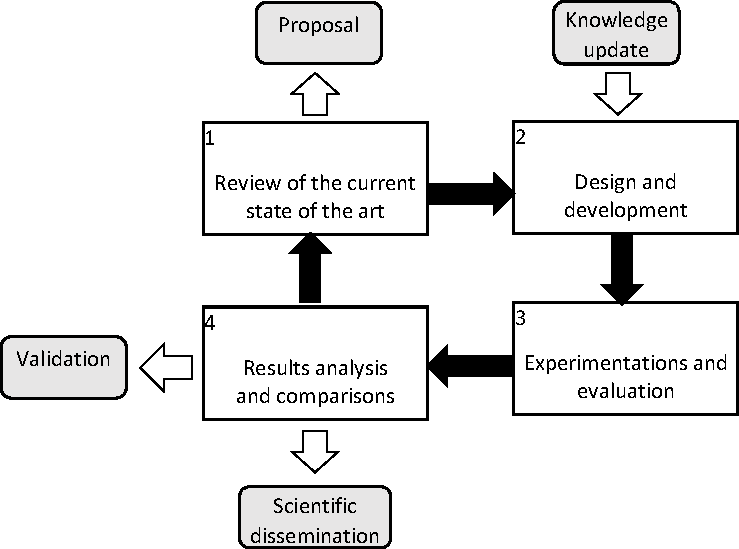
\includegraphics[width=.8\textwidth]{1_introduction/figures/fig_research-methodo.pdf}
    \caption{The research methodology of the thesis.}
    \label{ch1:research-emthodo}
\end{figure}

\begin{enumerate}
    \item \textbf{Review of the current state-of-the-art:}  The main objective of this phase is to investigate the state of the art related to the field under consideration to identify problems and/or challenges. To achieve this, the related bibliography is used, reviewing publications from the scientific community published in journals, and proceedings of international congresses. The knowledge acquired in this phase should lead to a proposal to address the identified challenges.

 \item \textbf{Design and development:} In this phase, a novel proposal to solve the identified challenges is designed and developed. To this end, previously acquired or updated knowledge is used to ensure that the solution is always up-to-date with the current state of the art.

\item \textbf{Experimentation and evaluation:} The goal of this phase is to test the proposals resulting from the previous step to a process of experimentation. To carry out this procedure, it is crucial to provide some criteria and evaluation methods with which the results will be compared in the subsequent phase. All these criteria and methods must be built using the knowledge acquired in the first stage of the methodology.

\item \textbf{Results analysis and comparison:} After carrying out experimentation, results must be analyzed and compared with those obtained in the state-of-the-art. At this point, it is needed to check if the results obtained are enough to address the challenges identified in the first phase. In such a case, another methodological cycle begins to approach the following challenge identified or to keep working with the challenge under consideration if it was not still solved. In this stage, conclusions must be drawn from analyses of results, and knowledge obtained must be materialized in scientific dissemination, either
through journals, or conferences.

\end{enumerate}









\section{Research Context} \label{ch1:research-context}

This research has received funding from the European Union’s Horizon 2020 research and innovation program under the Marie Skłodowska-Curie grant agreement Nº 665959. This research has also been funded and supported
by Deusto Smart Mobility Research Group, DeustoTech-Fundaci´on Deusto, the
Faculty of Engineering at the University of Deusto, (Spain). In addition, the Department of Systems and Computer Networks, Faculty of Electronics, Wrocław University of Science and Technology, (Poland).


During the second year of the Ph.D., an international research stay was made as
part of the research activities. The research stay was carried out at Wrocław University of Science and Technology (WUST) within the Department of Systems and Computer Networks. The stay lasted three months, from April to July 2019, under the supervision
of Dr. Michal Wo{\'{z}}niak. He is a supervisor of this research and a full professor at
Faculty of Electronics. The objective of the research stay was to
collaborate with international experts in the field of ensemble learning to share knowledge and get feedback from them. Therefore, it was possible to add more to the experiment design through several suggestions that later end with the dissemination of a scientific journal article.

In addition, participating in the 11th International Conference on Computer Recognition Systems (CORES), 2019, Poland, with a presentation of some results. Besides, participating in the 7th international student workshop, June 2019, Ladek Zdroj, Poland.  


\section{Structure of the Dissertation}
\label{sec:1_3_2_DissertationStructure}
The structure of the remainder of this thesis dissertation is outlined below.
\begin{description}	
	\item \textbf{Chapter~\ref{cha:2_background}} reviews background and related work about ML, supervised data mining, and ensemble data mining. In addition, we present a taxonomy of MCS. Furthermore, we discuss the importance of diversity and how to measure it. Finally, closing the chapter with the importance of soft computing.  
	
	\item \textbf{Chapter~\ref{cha:3_State-of-the-art}} reviews state-of-the-art  ensemble algorithms. This includes bagging-like, boosting, and gradient boosting ensembles. The revision includes different mechanisms to promote diversity in each algorithm. Following that, we group all the ensemble methods in a comparison table to show their properties. Finally, we spotlight on the role of metaheuristic algorithms (MA) to enhance the performance of MCS.  
	
	\item \textbf{Chapter~\ref{chapter4_training-set}} presents our first proposal to build an effective MCS from a reduced portion of the training data, and how to combine multi-decisions via SI algorithms. This chapter is therefore aligned with \emph{specific objective~1}.
	
	\item \textbf{Chapter~\ref{ch5_GUided_MCS_Pruning}} provides our second proposal to prune MCS via guided search.  We discuss how to merge ordering-based pruning metrics to gain what cannot be reached from any of them. The work presented in this chapter is therefore directly related to \emph{specific objective~2}. 
	
	\item \textbf{Chapter~\ref{cha:6_our_proposal}} presents an analysis of fast and accurate heuristic metrics for MCS pruning. The analysis shows how the performance of ensemble pruning metrics could be affected by the original ensemble size, the required subensemble size, the kind of individuals, and the number of classes. The work is directly related to \emph{specific objective~3}.
	
	\item \textbf{Chapter~\ref{cha:7_Conclusions}} revisits the main goal and specific objectives posted earlier. In this chapter, we summarise the main contributions of this thesis and outline possible future research.


\end{description}

%%%%%%%%%%%%%%%%%%%%%%%%%%%%%%%%%%%%%%%%%%%%%%%%%%%%%%%%%%%%%%%%%%%%%%%%


%%%%%%%%%%%%%%%%%%%%%%%%%%%%%%%%%%%%%%%%%%%%%%%%%%%%%%%%%%%%%%%%%%%%%%%%
